\documentclass{article}

\usepackage[utf8]{inputenc}

\usepackage{amsmath, bm}
\usepackage{graphicx}
\usepackage{amssymb}
\usepackage{float}
\usepackage{caption}
\usepackage{subcaption}
\usepackage{hyperref}
\usepackage{tikz}
\usepackage{layout}

\usepackage[margin=1in]{geometry}
\usepackage{listings}
\usepackage{xcolor}
\usepackage{color, colortbl}
\usepackage{textgreek}
\usepackage{mathrsfs}
\usepackage{savetrees}

\usepackage{titlesec}

\titleformat{\subsubsection}
  {\normalfont\selectfont}{\thesubsubsection}{1em}{}

\usetikzlibrary{calc}
\usetikzlibrary{angles,quotes} % for pic
\usetikzlibrary{patterns,snakes}
\usetikzlibrary{arrows}
\tikzset{>=latex} % for LaTeX arrow head

\setlength{\parskip}{\baselineskip}%
\setlength{\parindent}{0pt}%
\linespread{0.9}


\definecolor{codegreen}{rgb}{0,0.6,0}
\definecolor{codegray}{rgb}{0.5,0.5,0.5}
\definecolor{codepurple}{rgb}{0.58,0,0.82}
\definecolor{backcolour}{rgb}{0.95,0.95,0.92}

\lstdefinestyle{mystyle}{
    backgroundcolor=\color{backcolour},   
    commentstyle=\color{codegreen},
    keywordstyle=\color{magenta},
    numberstyle=\tiny\color{codegray},
    stringstyle=\color{codepurple},
    basicstyle=\ttfamily\footnotesize,
    breakatwhitespace=false,         
    breaklines=true,                 
    captionpos=b,                    
    keepspaces=true,                 
    numbers=left,                    
    numbersep=5pt,                  
    showspaces=false,                
    showstringspaces=false,
    showtabs=false,                  
    tabsize=2
}

\lstset{style=mystyle}



\begin{document}

\title{}
\author{lwp26}
\date{October 2024}
\maketitle 

\iffalse
\begin{abstract}
    \centering
    This report presents the development of a software tool to help solve constrained design optimization of a shell and tube heat exchanger.
    The software is developed in Python and uses LMTD and NTU methods to solve for the output parameters.
    Computational model is compared with experimental data 
    Various optimization algorithms were tested with constraints and the results are presented.
\end{abstract}
\fi

%-----------------------------------------------------------------------------------------
\section{Introduction}
%-----------------------------------------------------------------------------------------

\subsection{Objectives}
\begin{itemize}
    \item Determine the loss of stagnation pressure and the rate of
    change of momentum of the air through a turbine
    cascade by traversing the flow at exit
    \item Compare the rate of change of momentum of the air with
    the pressure force on a blade as obtained from the
    measurement of the static pressure distribution around it
    \item Examine the limitations of the measurements in the light
    of calculations and correlations.
\end{itemize}

\subsection{Setup}

\begin{figure}
    \centering
    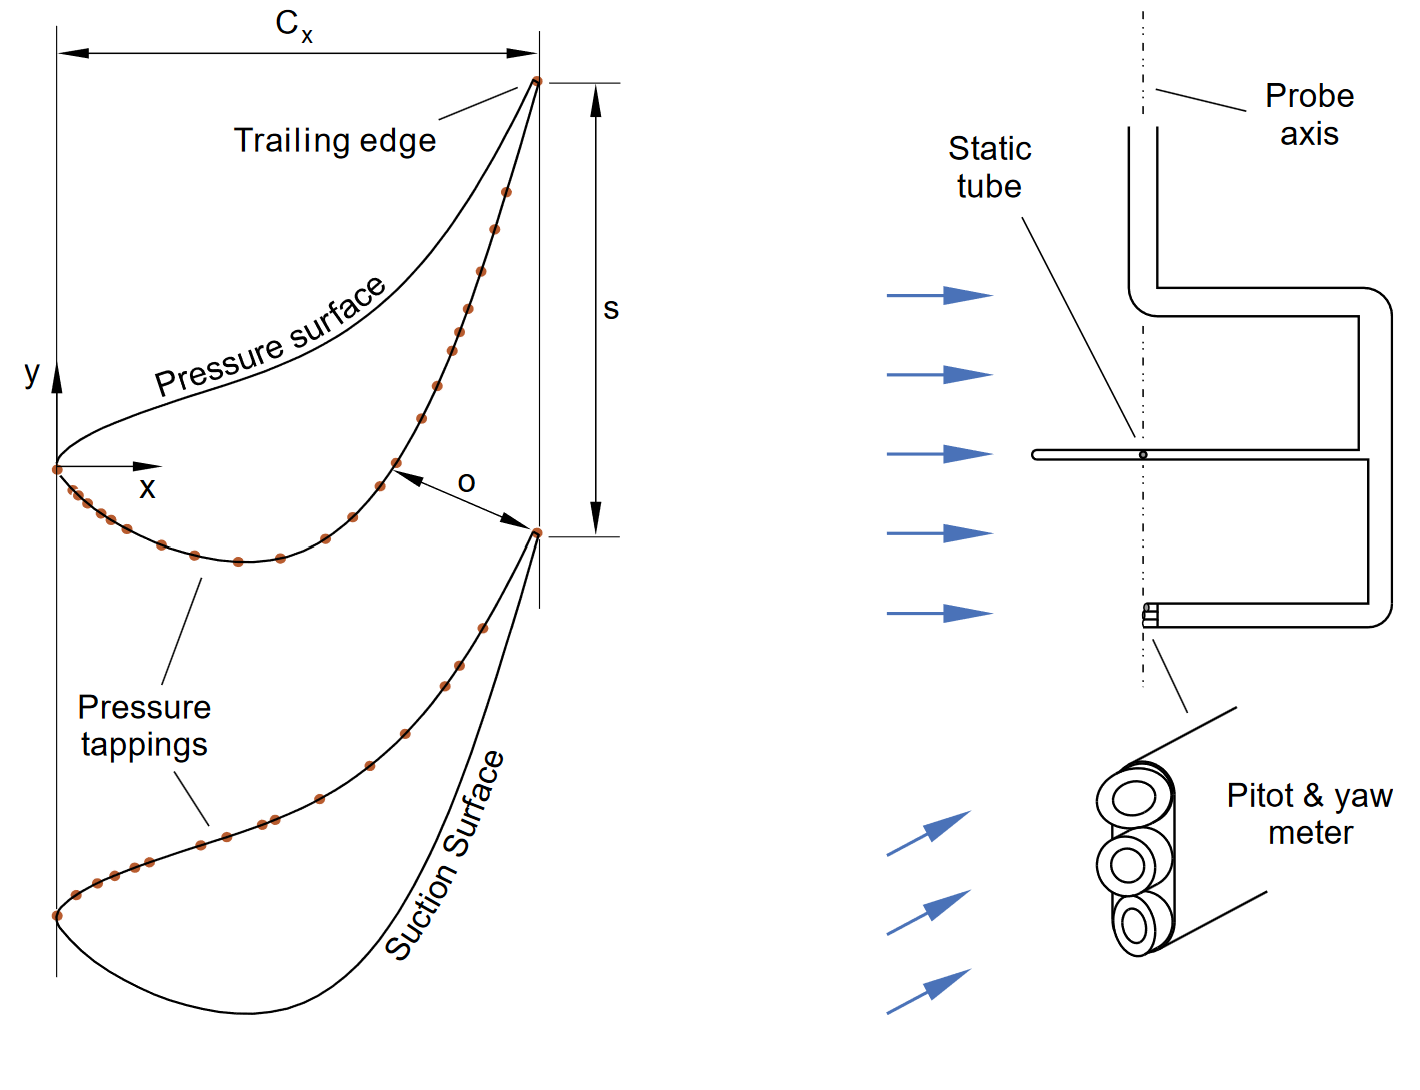
\includegraphics[width=0.8\textwidth]{figures/tappings_and_yawtube.png}
    \caption{Pressure tapping locations on the blade and and schematic of the yaw tube.}
    \label{fig:setup}
\end{figure}

\section{Results}

\begin{figure}[H]
    \centering
    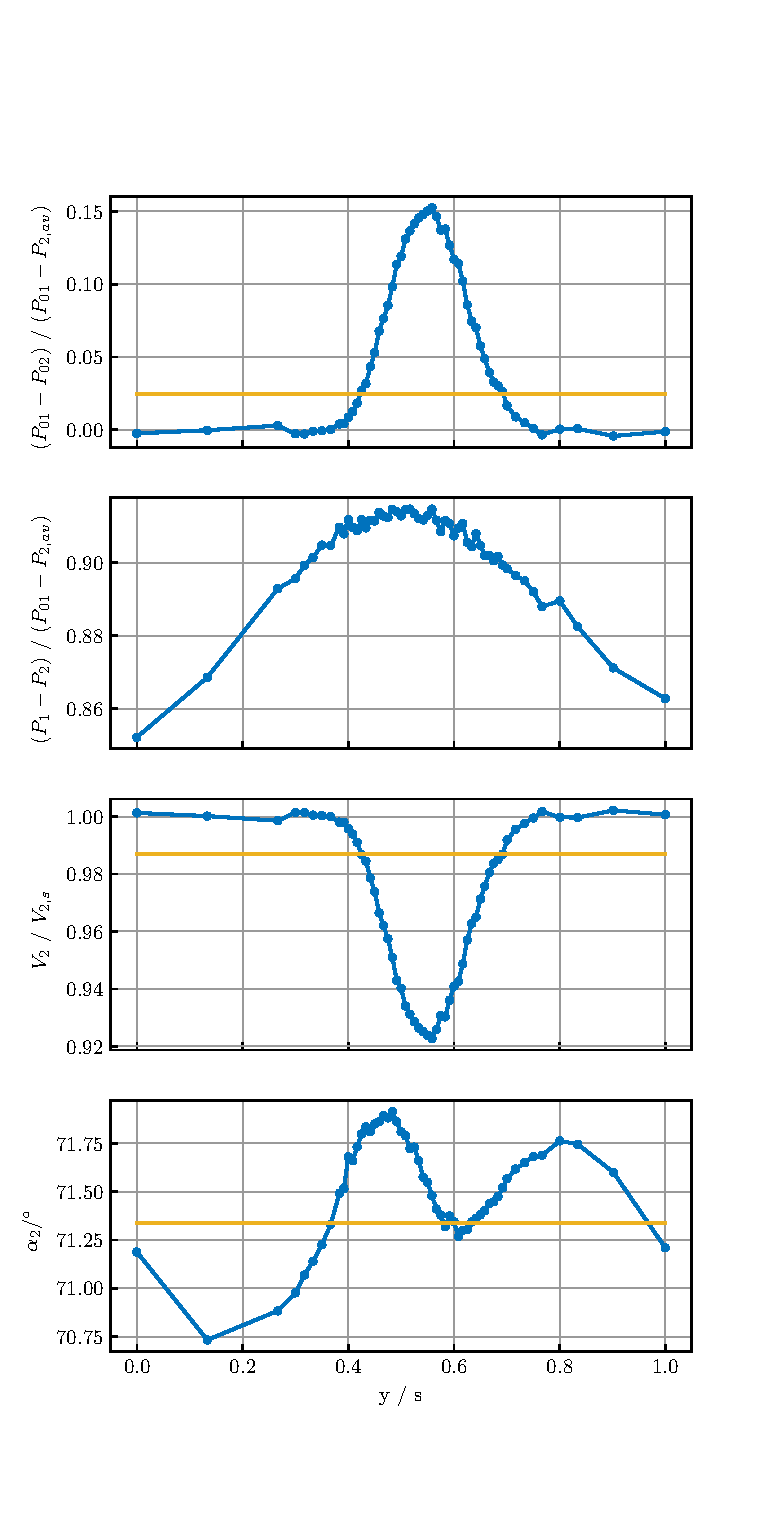
\includegraphics[width=0.6\textwidth]{figures/wake_plot.eps}
    \caption{wake plot}
    \label{fig:wake_plot}
\end{figure}

\begin{figure}[H]
    \centering
    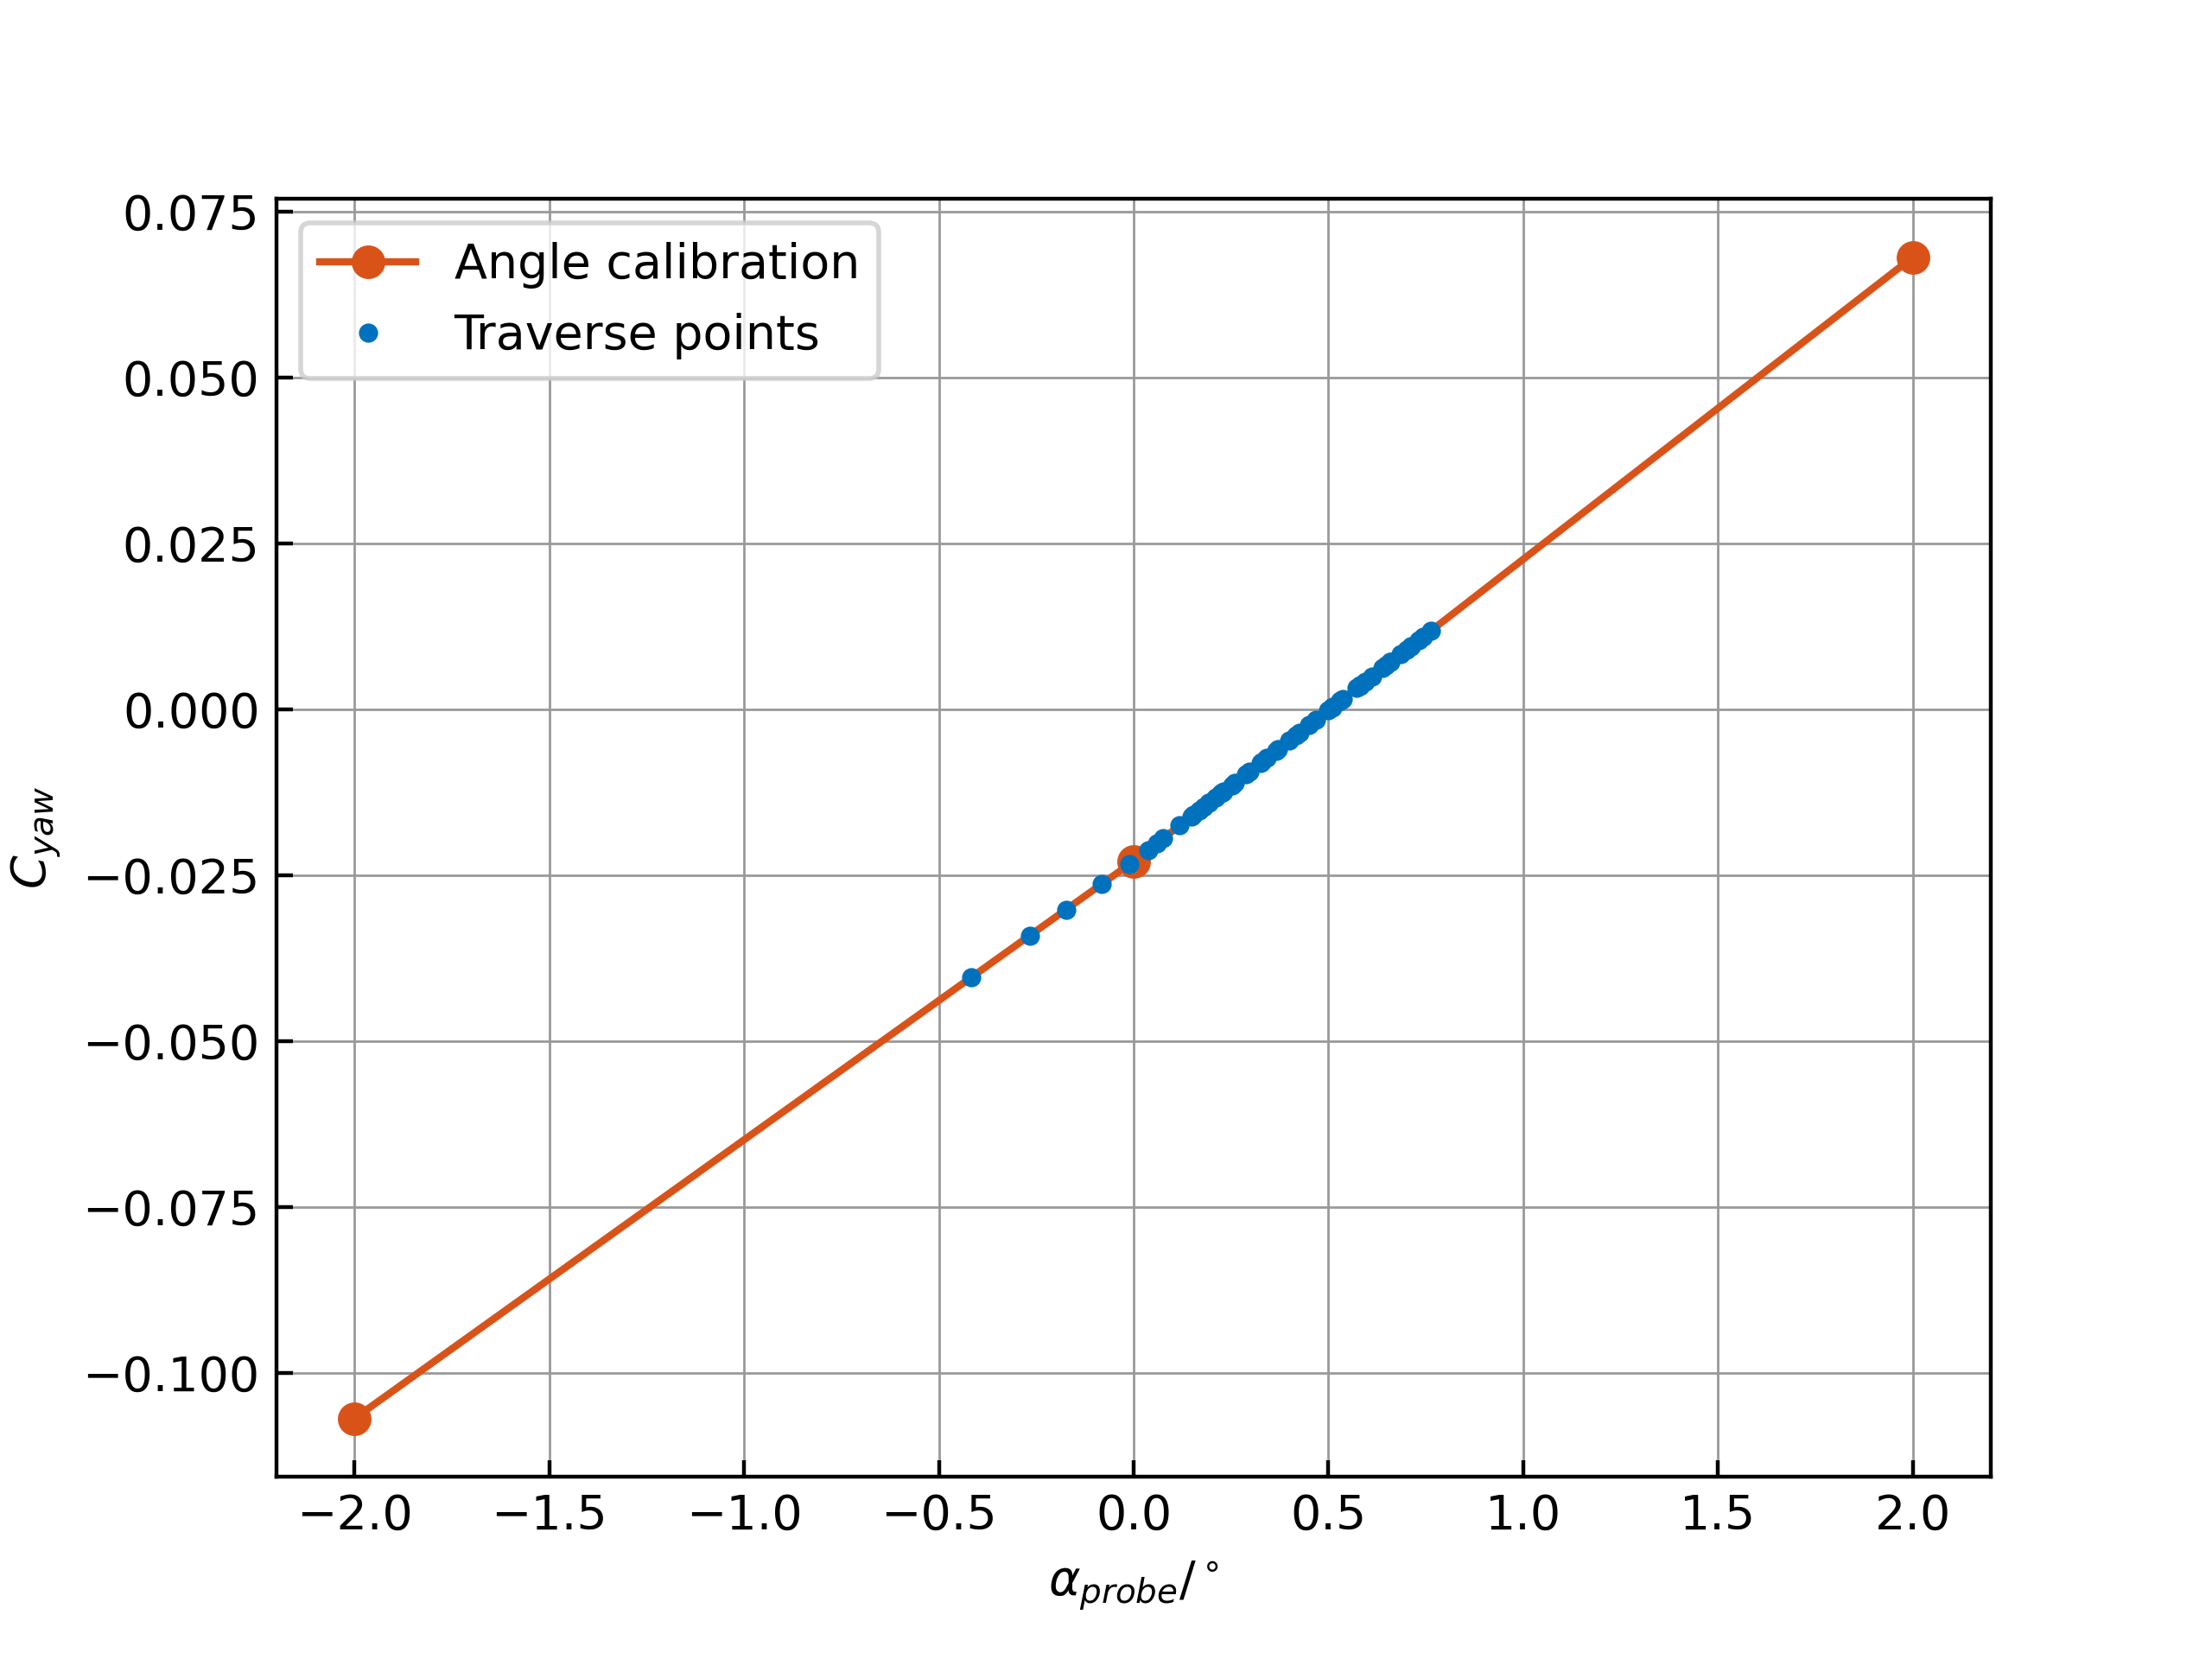
\includegraphics[width=0.8\textwidth]{figures/yaw_plot.png}
    \caption{yaw plot}
    \label{fig:yaw_plot}
\end{figure}

\begin{figure}[H]
    \centering
    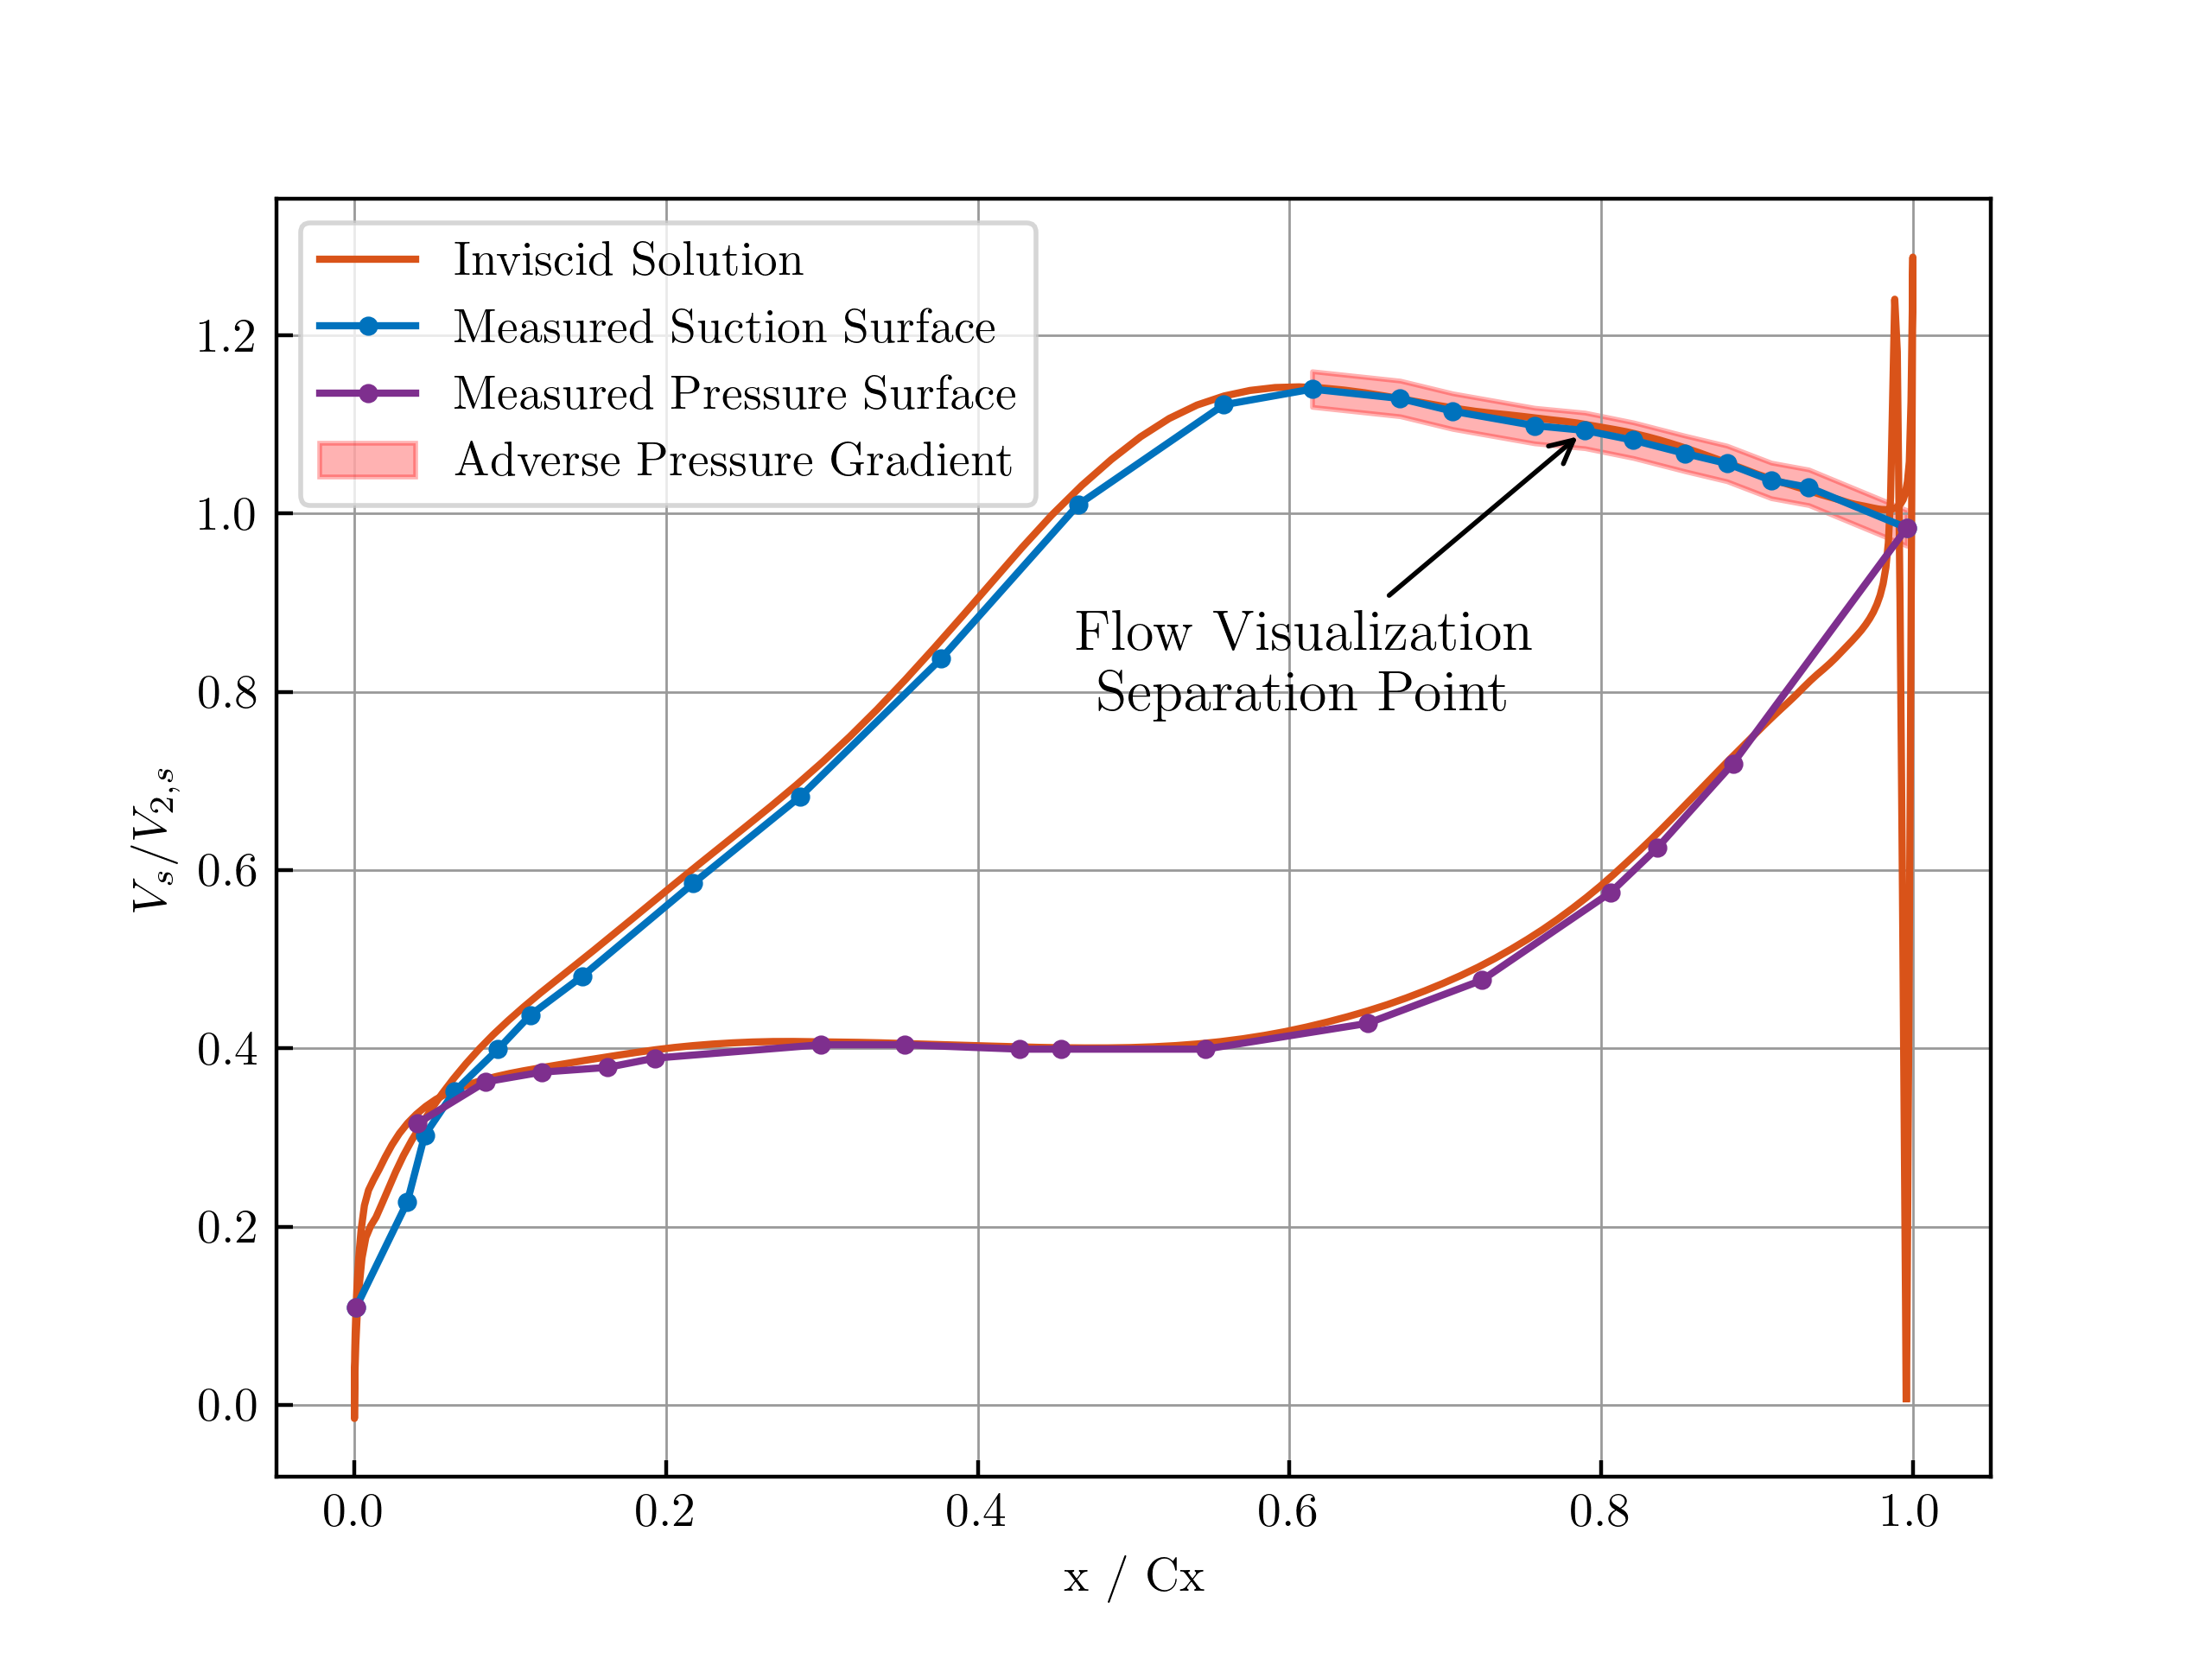
\includegraphics[width=0.8\textwidth]{figures/lift_plot.png}
    \caption{lift plot}
    \label{fig:lift_plot}
\end{figure}
\begin{figure}[H]
    \centering
    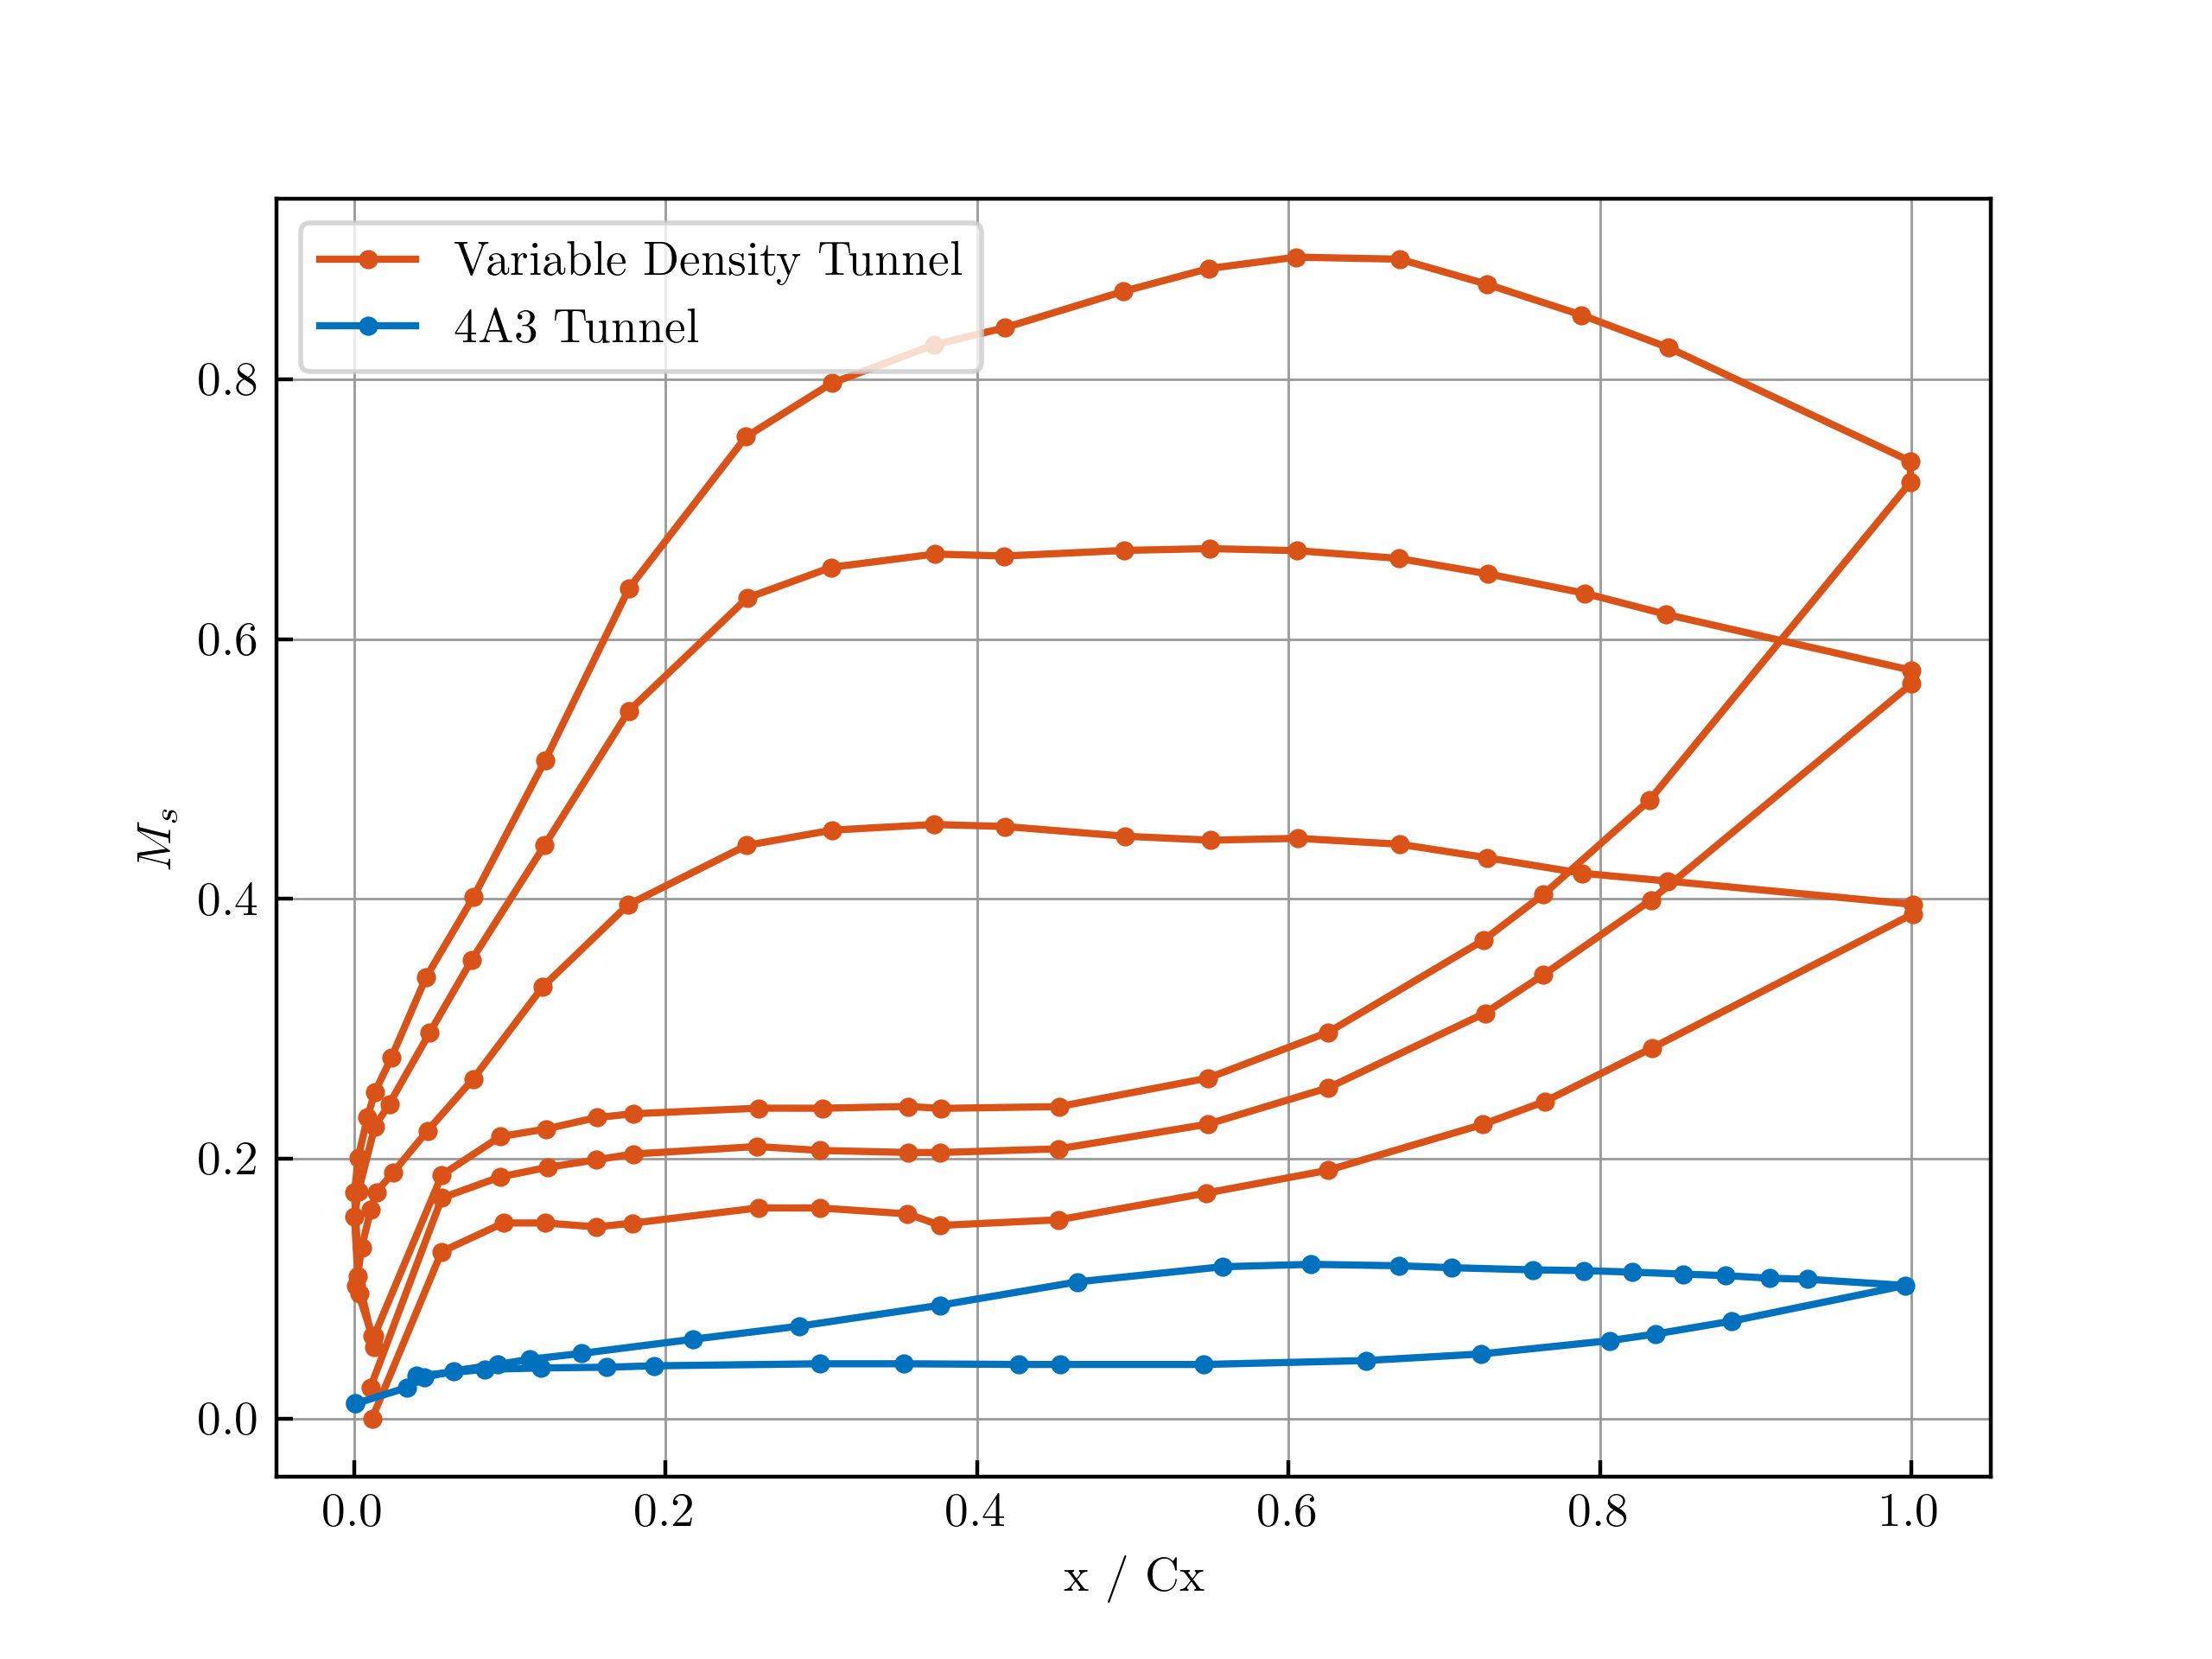
\includegraphics[width=0.8\textwidth]{figures/mach_plot.png}
    \caption{mach plot}
    \label{fig:mach_plot}
\end{figure}
\begin{figure}[H]
    \centering
    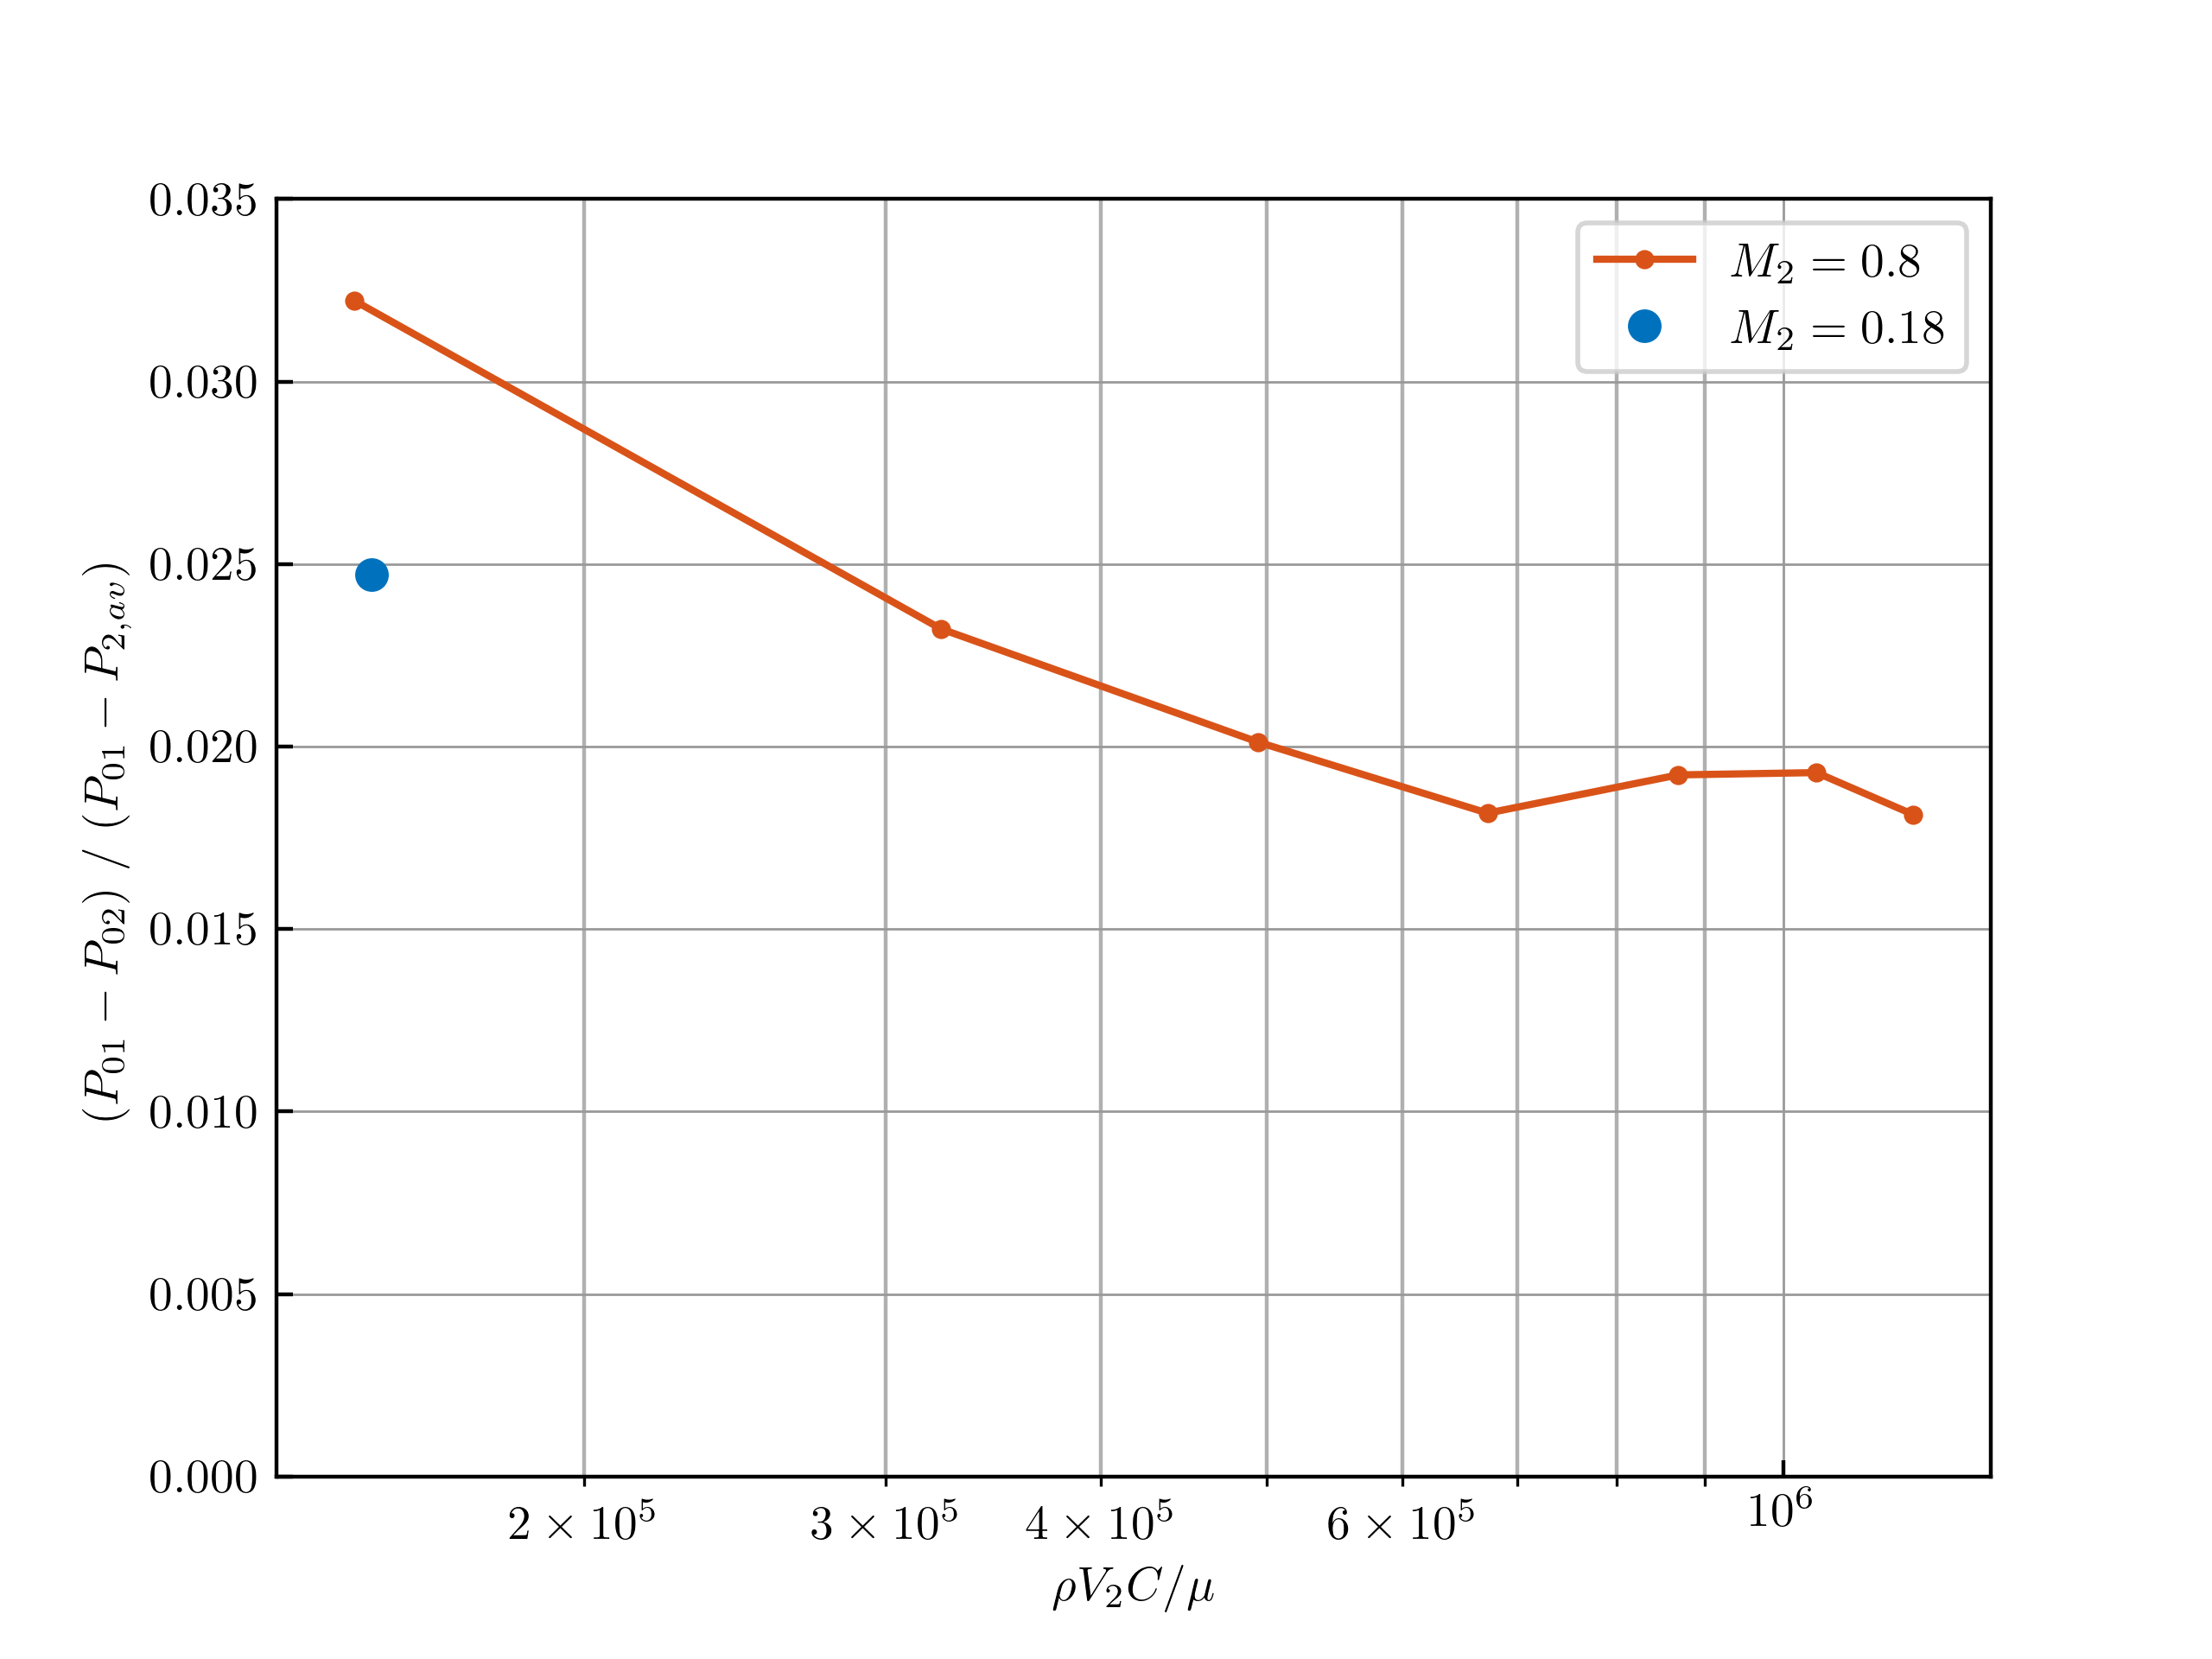
\includegraphics[width=0.8\textwidth]{figures/reynolds_plot.png}
    \caption{reynolds plot}
    \label{fig:reynolds_plot}
\end{figure}

\begin{figure}[H]
    \centering
    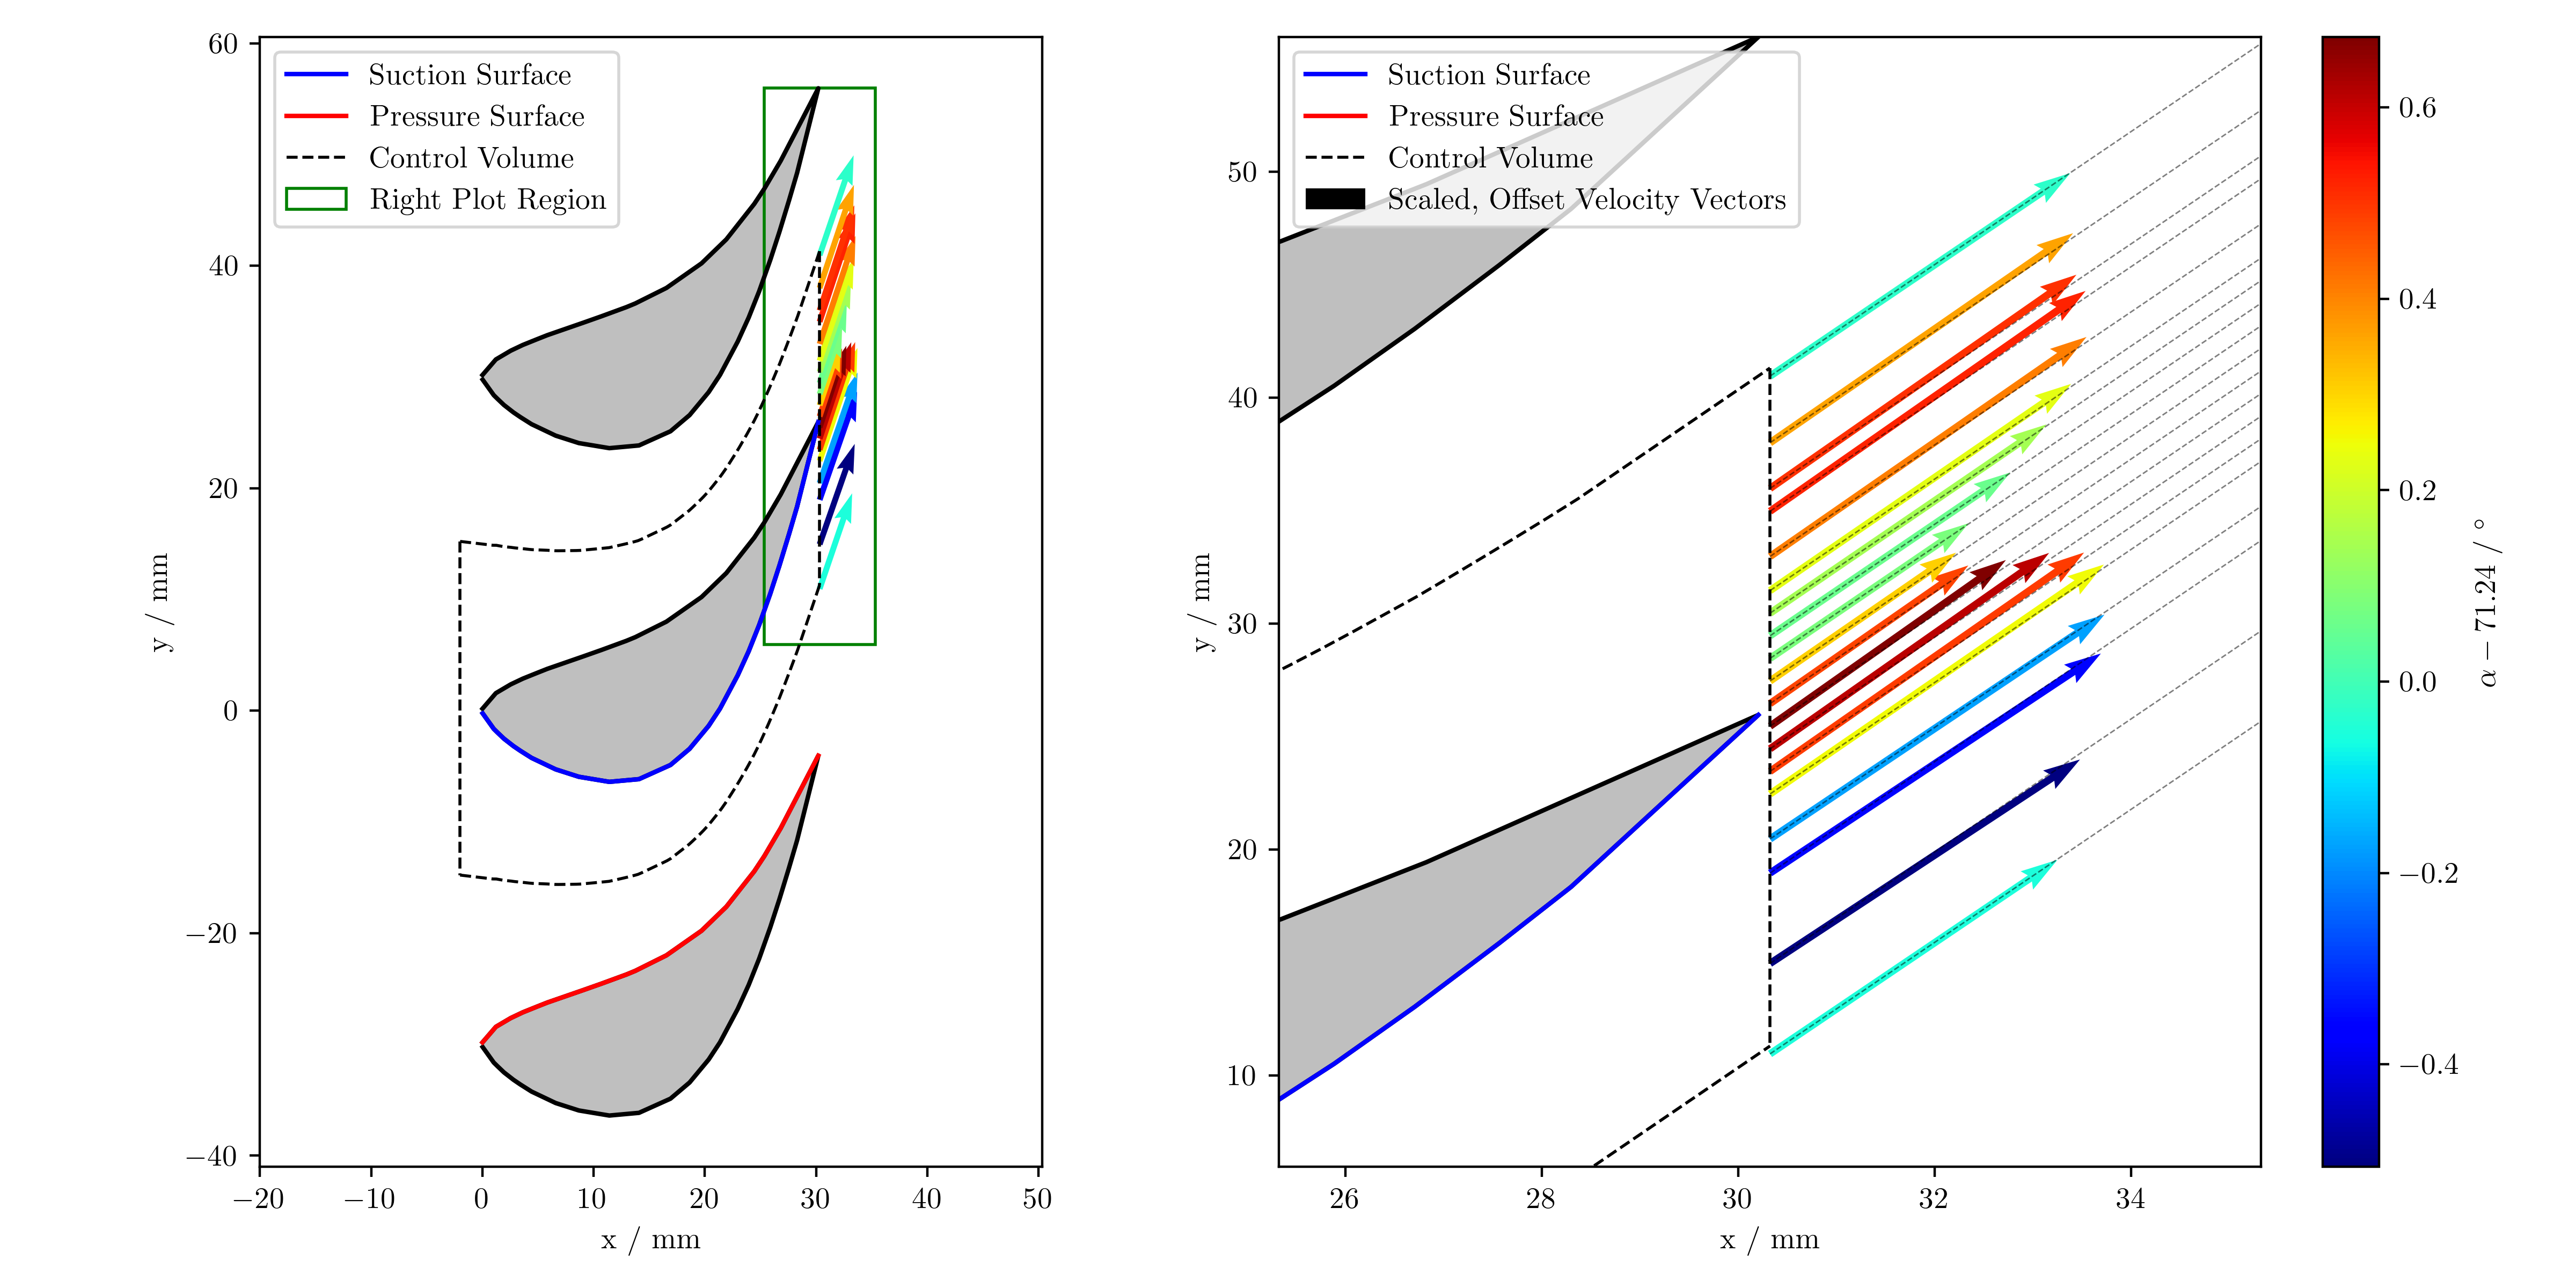
\includegraphics[width=0.8\textwidth]{figures/quiver_plot.png}
    \caption{Quiver Plot of Measured Velocity Vectors. The lengths are offset to be $V-0.9V_\text{min}$}
    \label{fig:quiver_plot}
\end{figure}


\section{Discussion}

\subsection{General}

\subsubsection{ Assume isentropic flow to estimate the change of density from the measurements of
upstream and downstream static pressure. Can the flow be regarded as incompressible?}

\begin{equation}
    \frac{P}{\rho^\gamma} = \text{const}
\end{equation}

Upsteam of cascade, $P_{0in} = 105.1$ KPa , $P_{in} = 104.8$ KPa \\
Downstream of cascade,  $P_a = 102.8$ KPa , $\rho = 1.16$ kg/m3

For clarity we will use the subscript 1 to denote upsteam of the cascade and 2 to denote downstream of the cascade.
To calculate the density upstream of the cascade, $\rho_1$, we will assume the isentropic relation.

\begin{equation}
    \rho_1 = \rho_2 \left( \frac{P_1}{P_2} \right)^\frac{1}{\gamma}
\end{equation}
Which gives $\rho_1 = 1.176$ kg/m3.

This means that the density change is 1.4\% which is likely of similar order to the error in the measurements.
Hence, the flow can and will be regarded as incompressible from this point on. %REVISIT

\subsubsection{Using the data you have acquired, evaluate the following quantities at the first
measurement point in your traverse, which should be in the freestream between the wakes?}

\subsubsection{the inlet velocity to the cascade,}
$P_{01} = P_1 + \frac{1}{2} \rho V_{1}^2$
Where $V_1$ is the inlet velocity to the cascade and the only unknown.\\
This is found to be $V_1 = 22.7$ m/s.

\subsubsection{the exit velocity,}
Between the wakes, the flow is assumed to be isentropic and so $P_{01} = P_{02}$.
The pressure here is $P_a$ as the flow is exiting to the atmosphere.
$P_{02} = P_a + \frac{1}{2} \rho V_{2}^2$
Where $V_2$ is the exit velocity from the cascade and the only unknown.\\
This is found to be $V_2 = 62.97$ m/s.

\subsubsection{the difference between the inlet and exit static pressures.}

Difference between inlet and exit static pressures is $P_1 - P_a = 2.0$ KPa

Explain why the velocity rises and the static pressure falls across the cascade.

The flow is turned through an angle to a smaller area, which by mass conservation, must increase the velocity.
In the free stream, this is done isentropically and so the static pressure must fall to conserve energy.

\subsection{Exit Traverse}
\subsubsection{The script shows a series of graphs showing the normalised variation of the quantities
}

\begin{align*}
    \text{Stagnationg pressure loss} \quad & \frac{P_{01} - P_{02}}{P_{01} - P_{2,\text{av}}} \\
    \text{Static pressure} \quad & \frac{P_{1,\text{av}} - P_2}{P_{01} - P_{2,\text{av}}} \\
    \text{Exit velocity over isentropic velocity} \quad & \frac{V_2}{V_{2\text{s}}} \\
    \text{Exit yaw angle} \quad & \alpha_2
\end{align*}

across one pitch of the flow behind the blades. Note that the denominators as well as the
numerators in the coefficient correspond to measurements taken at the same time as the probe
pressures are taken. This minimises the effects of small changes in tunnel speed upon the data.

$P_{1,\text{av}}$ is the average of five cascade inlet endwall static pressure tappings shown in Fig. ?

$P_{2,\text{av}}$ is the average exit pressure from the cascade, in this experiment it is equal to the
atmospheric pressure


Explain why we use $(P_{01} - P_{2,\text{av}})$ as the denominator for the first two quantities above in
preference to $(P_{01} - P_{1,\text{av}})$ or $(P_{02} - P_{2,\text{av}})$?

$P_{01}$ remains constant across the cascade, and $P_{2,\text{av}}$ is the exit static pressure averaged over the cascade.
This provides a constant reference for the normalisation of the quantities.
$ P_{02} \le P_{01} $ and $P_{02} > P_{2,\text{av}}$  % REVISIT


Comment on the shape of all the curves and the magnitude of any variations. Explain the origin
of the important features

Figure \ref{fig:wake_plot} shows the variation of the quantities defined above, in their respective order, across a single blade section.
The traverse covers a whole blade pitch, starting below in the free stream and moving up through the blades wake and into the free stream above the blade.

The first graph shows the stagnation pressure loss coefficient, which is observed to be near zero far from the blade, in the free stream.
This reaffirms our assumption that the flow behaves isentropically in the free stream.
However, in the wake of the blade we see it rise sharply to a peak of about 0.15.
The width of this peak is about 30\% of the pitch of the blade.
Perhaps the most interesting observation is that the center of the wake is offset about 5\% of the pitch from the trailing edge location.

The second graph showing static pressure 
The measurements in the wake can be seen to be noisy, which could indicate unsteady boundary layer interactions.
However, on further inspection it is $P_1$ that is noisy, which means what? % REVISIT
% graph dips down either side in the free stream, suggesting P2 is higher here than in the middle.
% This doesnt make sense though as the velocity in free steam is higher
% need to investigate this further

The third graph shows the exit velocity over the isentropic free stream velocity.
This is seen to be near unity in the free stream, as expected.
In the wake, the velocity is seen to drop to about 92\% of the free steam isentropic value.

This is due to the boundary layer separation and the formation of the wake.

The final graph shows the exit yaw angle.
This initially starts, in the free stream, about 1 degree below the metal blade angle $\chi_2$.
Close to the suction surface, the flow angle increases to higher than metal blade angle.
This then reduces down to a value similar to the metal blade angle at a height similar to the wake peak.
Then, above the wake the flow angle again is higher than the metal blade angle, before decreasing to value seen in the free steam.


\subsubsection{The probe is used to measure the flow angle via the yaw coefficient defined as
}

\begin{equation}
    C_\text{yaw} = \frac{P_\text{left} - P_\text{right}}{P_0 - P}
\end{equation}
Explain how the initial calibration of the probe is used to determine the flow angle across the
pitch of the passage using the yaw coefficient. Over what range is the calibration valid?

The pressures $P_\text{left}$ and $P_\text{right}$ stagnate the components of velocity normal to them.?? % REVISIT
The difference in these pressures  produce a term proportional to $\rho V^2 \sin \delta$, which when divided by the dynamic pressure gives the yaw coefficient.
For small angles the yaw coefficient will be proportional to the angle of the flow which can be seen in the calibration plot \ref{fig:yaw_plot}.
The calibration constant is found by placing it at known angles, $\pm 2^\circ$ to the flow in the free stream.
Then small angles of the flow can be determined by the yaw coefficient.

\subsubsection{Besides the plots, the script also calculates various average quantities that are printed
to screen. One of these is the mass averaged stagnation pressure loss coefficient as defined by}

% bibliography

\begin{equation}
    Y_p = \frac{p_{01} - \overline{p_{02}}}{p_{01} - p_{2,av}} = \frac{\int_{-s/2}^{s/2} \rho_2 V_{x2} \frac{p_{01} - p_{02}}{p_{01} - p_2} \, dy}{\int_{-s/2}^{s/2} \rho_2 V_{x,2} \, dy}
\end{equation}

Explain how mass averaging is used and in where it is appropriate to apply this treatment of
data reduction

The mass flow weighted average is used to obtain a more accurate representation of the overall flow from a non uniform flow field.
Changes in flow properties such as energy and momentum are governed by the mass flow rate, making it the most appropriate quantity to average over.

This averaged value was found to be $Y_{p,av} = 0.0247$

\subsubsection{Use a control volume analysis and the average values from the exit traverse to determine
the axial and tangential force on a blade. Hence, evaluate the force coefficients
}
The pressure and momentum forces on the blade are calculated from the steady flow momentum equation of the control volume in figure \ref{fig:quiver_plot}.

\begin{equation}
    F_x =  F_{x,m,2} - F_{x,m,1} + F_{x,p,1} - F_{x,p,2} \quad \& \quad F_y =  F_{y,m,2} - F_{y,m,1}
\end{equation}

The subscripts $m$ and $p$ denote the momentum and pressure forces respectively, and the subscripts 1 and 2 denote the inlet and exit of the control volume.
There are no resulting pressure components in the y-direction due to infinite cascade symmetry.
This gives values of $F_x = 59.784$ N and $F_y = 41.042$ N.

\begin{equation}
    Z_x = \frac{F_x}{0.5 \rho_2 V_2^2 h C_x} \quad \& \quad Z_y = \frac{F_y}{0.5 \rho_2 V_2^2 h C_x}
\end{equation}

where $h$ is the span of the blade and $C_x$ is the axial chord. Comment on the relative magnitudes
of $Z_x$ and $Z_y$. How would your answers change if the traverse plane were moved further
downstream? What role do viscous forces on the blades play in your analysis?

Using the value of $V_2s = 62.97$ m/s, $C_x = 30.323$ mm and span $h=101.6$ mm gives $Z_x = 8.438$ and $Z_y = 5.793$.
These force coefficients are of similar magnitude, with more axial force than tangential force.
If the traverse plane were moved further downstream, more momentum mixing would occur and the quantities would be more similar.
Viscous forces on the blades \dots

\subsubsection{The script evaluates the average pitchwise exit flow angle using the relationship
}
\begin{equation}
    \tan (\overline{\alpha}_2) = \frac{\text{y momentum at 2}}{\text{x momentum at 2}} = \frac{\rho V_{x,2}V_{y,2}}{\rho V_{x,2}^2} \label{eq:alpha2}
\end{equation}
The inviscid flow calculation predicts that the exit flow angle should be $71.6^\circ$. Compare the
measured value of $\overline{\alpha}_2$ with the predicted vaue. Comment on any differences.

The angle obtained in our experiment, $\overline{\alpha}_2 = 71.34^\circ$ is 0.36\% smaller than the value predicted by the inviscid flow calculation.
This small difference can cause significant change in $tan(\overline{\alpha}_2)$ and $1/cos(\overline{\alpha}_2)$, shifting away from the optimum design point.
It is however, difficult to determine the cause of such a small difference.
Along the traverse, $\alpha$ changes significantly over the span. In the suction surface side of the free stream, the angle is below the average, while on the pressure surface side of the free stream, the angle is above the average.
There is a trough, of which the center is offset 0.05s above the pressure loss coefficient peak. The value at the bottom of the trough is the average.

% reasons for x momentum at 2 being higher for viscous flow than inviscid flow:
% boundary layer growth restricting the inside flow area, increasing the velocity
% 
% reasons for y momentum at 2 being lower for viscous flow than inviscid flow:


A simple one-dimensional analysis gives the approximate relationship between the exit flow angle $\alpha_2$, the throat $o$, and the pitch $s$ as
\begin{equation}
    \cos (\overline{\alpha}_2) = \frac{o}{s}
\end{equation}
Compare your measurements and the value given by this equation. Comment on any
differences.
\begin{equation}
    \cos^{-1}\left( \frac{o}{s} \right) = 71.123^\circ
\end{equation}
The measured angle is much greater than the value predicted by this equation.
This could occur 

\subsubsection{The axial velocity ratio of the cascade is determined from the equation
}
\begin{equation}
    \text{AVR} = \frac{\overline{V_{x,2}}}{V_{x,1}} = \frac{1}{s V_{x,1}} \int_{-s/2}^{s/2} V_{x,2} \, dy
\end{equation}

If the flow were truly two dimensional and truly incompressible, then the axial velocity ratio
would be unity since, at mid-span, the mass flow per unit area at inlet would be the same as
that at exit. Discuss whether density changes across the cascade are enough to describe any
differences to unity you observe and, if not, explain what else may be responsible?

AVR = $0.939$ which shows a 6.1\% reduction in the axial velocity.
The reduction in density of 1.4\% means that, if we account for compressibility, the outlet axial velocity should actually be higher than the inlet.
This means that there must be 


\subsection{Blade Surface Pressure Distribution}

The same script will assist you with the reduction of the static pressure data.
\subsubsection{The script evaluates the static pressure coefficient $C_p$ and the isentropic velocity for
each of the pressure tappings on the blade surface. The coefficient $C_p$ is defined as}

\begin{equation}
    C_p = \frac{P_{01} - P}{P_{01} - P_2}
\end{equation}

where P is the static pressure on the blade surface. The isentropic velocity
$V_s$, which may be
regarded as the velocity in the flow just outside the boundary layer, is normalised by the
isentropic exit velocity
$V_{2s}$ so that the ratio is defined as

\begin{equation}
    \frac{V_s}{V_{2s}} = \sqrt{\frac{P_{01} - P}{P_{01} - P_{2,av}}} = \sqrt{C_p}
\end{equation}
Mark the pressure and suction surfaces and any regions of adverse pressure gradient.

The adverse pressure gradients are shown on figure \ref{fig:lift_plot}.

A prediction of the isentropic blade-surface velocity distribution with the cascade at its
design condition has been obtained using a boundary element CFD code. This solves the
equation for potential flow through the cascade. The prediction for the design condition is
reproduced by the script for comparison with the experimental data.

\subsubsection{Diffusion factors are often used in turbine design to quantify flow deceleration. It is
reasoned that profile losses in a turbine primarily depend on the amount of diffusion on the
suction surface. Hence, the most commonly used 'local' diffusion factor is defined as
}

\begin{equation}
    D = \frac{V_\text{max} - V_2}{V_\text{max}}
\end{equation}
where
$V_\text{max}$ is the maximum suction surface velocity and
$V_2$ is the exit velocity. Calculate the
diffusion factor, D, from your cascade measurements.

\subsubsection{On the plot of the velocity distribution, indicate the location of any separation lines seen
in the flow visualisation.}


\subsubsection{Find the fraction by which the surface velocity has decreased from the maximum value
to the separation point. For a laminar boundary layer, this is typically 5-8%. For a turbulent
boundary layer, it is much more. What state is the boundary layer in at the trailing edge, laminar
or turbulent, separated or attached?}


\subsubsection{Comment on any differences between the measured and predicted velocity
distributions.}


\subsubsection{The script also integrates your measured pressure distribution to determine the pressure
blade force per unit span in the y-direction and x-direction. It then evaluates the force
coefficients $Z_x$ and $Z_y$ and these are printed to screen.
Compare the pressure blade force coefficients with the values indicated by the results of your
exit traverse and comment on any discrepancy.}


\subsection{Effect of Reynolds number}

The Reynolds number is defined as
\begin{equation}
    Re = \frac{\rho V_2 C}{\mu}
\end{equation}

The script shows how the profile loss of the cascade varies with Reynolds number at an exit
Mach number of 0.8. These results were obtained when the same cascade hardware was tested
in the high-speed variable density tunnel at the Whittle Laboratory.

\subsubsection{Compare your measurements with the other values. What do you conclude about the
effect of Mach number?}


\subsubsection{Figure 3 shows the results of flow visualisation experiments at high and low Reynolds
numbers. The effect of Reynolds number on the behaviour of the boundary layer can be seen
near the trailing edge. Suggest reasons for the shape of the relationship between loss and
Reynolds number that you plotted.}



\subsection{Effect of Mach number}
The script shows surface isentropic Mach number distributions for this cascade at different
values of the nominal exit Mach number (M2 = 0.39 to 0.75). Comment on the variation of
diffusion factor with Mach number. Would these blades be more suitable for high or low Mach
numbers?


\begin{thebibliography}{9}


  \bibitem{handout}
  J. V. Taylor
  \emph{Turbine Cascade Aerodynamics Handout}
  University of Cambridge,
  October 2024.

\end{thebibliography}

\end{document}